%%%%%%%%%%%%%%%%%%%%%%%%%%%%%%%%%%%%%%%%%
% a0poster Portrait Poster for LiRI/UZH
% LaTeX Template
% Version 1.0 (22/06/13)
% Version 2.0 (08/04/22)
%
% The a0poster class was created by:
% Gerlinde Kettl and Matthias Weiser (tex@kettl.de)
% adapted by Danny McDonald for LiRI/UZH (mcddjx@gmail.com)
%
% License:
% CC BY-NC-SA 3.0 (http://creativecommons.org/licenses/by-nc-sa/3.0/)
%
%%%%%%%%%%%%%%%%%%%%%%%%%%%%%%%%%%%%%%%%%

\documentclass[a0,portrait]{a0poster}

% control margins here
\usepackage{geometry}
 \geometry{
 a0paper,
 left=5cm,
 top=4.5cm,
 right=5cm,
 bottom=4.5cm
 }
\addtolength{\textwidth}{4.5cm} % width of text can be adjusted if margins above are adjusted

\usepackage{multicol} % This is so we can have multiple columns of text side-by-side
\columnsep=3em % This is the amount of white space between the columns in the poster
\columnseprule=0pt % This is the thickness of the black line between the columns in the poster

% UZH colours
\usepackage[svgnames]{xcolor}
\definecolor{primary}{RGB}{0, 0, 0}
\definecolor{secondary}{RGB}{90, 90, 90}
\definecolor{section}{RGB}{50, 50, 50}
\definecolor{conclusion}{RGB}{240, 240, 240} % the conclusion box colour

\usepackage{ifthen} % needed to stop horizontal line above 'Conclusions' section
\usepackage{graphicx} % Required for including images
\graphicspath{{figures/}} % Location of the graphics files
\usepackage{mwe,tikz}\usepackage[percent]{overpic} % overlay your photo over the background
\usepackage{booktabs} % Top and bottom rules for table
\usepackage[font=small,labelfont=bf]{caption} % Required for specifying captions to tables and figures
\usepackage{amsfonts, amsmath, amsthm, amssymb} % For math fonts, symbols and environments
\usepackage{wrapfig} % Allows wrapping text around tables and figures

\usepackage{fontspec} % custom fonts
\defaultfontfeatures[Palatino]
{
    Extension = .ttf,
    UprightFont = font/LT_41167,
    BoldFont = font/LT_41169,
    ItalicFont  = font/LT_41168,
    BoldItalicFont = font/LT_41170,
}
\defaultfontfeatures[TheSans]
{
    Extension = .otf,
    UprightFont = font/TheSans-LP5Plain,
    BoldFont = font/TheSans-LP7Bld,
    ItalicFont  = font/TheSans-LP5PlainIT,
    BoldItalicFont = font/TheSans-LP7BldIT,
}
\setmainfont{TheSans} % choose your font here
\usepackage[onehalfspacing]{setspace} % remove for single spacing
\usepackage{tcolorbox} % for the conclusions box
\usepackage{blindtext} % you can remove this once you add your content
\usepackage[export]{adjustbox} % allow floating a graphic right
\usepackage{titlesec} % customising section titles
\usepackage{needspace} % prevent break between line and section title
\usepackage{nameref} % package and command to get the name of the current section (for ifthen)
\usepackage{url} % for URLs in bibliography

\begin{document}

% define how our section titles will look (with ruled line)
\titleformat{\section}
  {\needspace{1\baselineskip}\sectionrule\huge\bfseries}
  {\color{section}\thesection.}
  {1em}
  {\color{section}}

% draw horizontal line before section unless it is conclusions (if you change name of Conclusions, you should
% also change it here too so it is recognised and the line suppressed
\makeatletter
\newcommand{\sectionrule}{%
 \ifthenelse{\equal{\@currentlabelname}{Introduction} 
 \OR \equal{\@currentlabelname}{Experiments} 
 \OR \equal{\@currentlabelname}{Conclusions}}
 % use the below line instead of the above if conclusions is a section*
 % \ifthenelse{\equal{\@currentlabelname}{}}
  {}
  {\vspace*{-\baselineskip}
   \vrule height 1pt depth 1pt width \linewidth\vskip0.4pt
   \bigskip}%
}
\makeatother


%----------------------------------------------------------------------------------------
%	POSTER HEADER 
%----------------------------------------------------------------------------------------
%\title{Creating a \LaTeX{} poster template matching UZH specifications for LiRI presentations}
\title{Curriculum Induction for Safe Reinforcement Learning}

% the top logo (in english!) and unit title
\noindent
\begin{minipage}{.25\linewidth}
\centering
 
\includegraphics[width=5cm]{figures/tu_berlin.png}
\end{minipage}
\begin{minipage}{.50\linewidth}
\centering
 \color{secondary}\huge{\textbf{Neural Information Processing Project}}
\end{minipage}
\begin{minipage}{.25\linewidth}
\centering
 
\includegraphics[width=4.5cm]{figures/ni_group.pdf}
\end{minipage}
\vspace{2em}

% The header is divided into two boxes, on the left is the text and on the right is the image
\begin{minipage}[b][][t]{\linewidth}
\vfill
\makeatletter
\centering{\fontsize{92pt}{100pt}\selectfont\color{primary}\textbf{{\@title}}\par}
\makeatother
\color{Black}
\vspace{1cm}
%\Huge\textit{Subtitle goes here}\\[2.4cm] % Subtitle if it exists
Marvin Sextro\textsuperscript{1} and Jonas Loos\textsuperscript{1}\\
\vspace{0.2cm}
\textsuperscript{1}Technical University of Berlin
\end{minipage}


\vspace{1cm}

%----------------------------------------------------------------------------------------
%	POSTER BODY
%----------------------------------------------------------------------------------------

\begin{multicols}{3} % This is how many columns your poster will be broken into

%----------------------------------------------------------------------------------------
%	INTRODUCTION
%----------------------------------------------------------------------------------------

\section{Introduction}
\setlength{\parindent}{0pt}  % remove indentation at the beginning of paragraphs
\large

\subsection{Key Ideas$^\text{2}$}

\begin{itemize}
    \item A teacher trains a student to solve a task
    \item The teacher keeps the student safe during training
    \item For this, the teacher is given a set of pre-defined interventions and learns to apply them optimally\\$\rightarrow\emph{curriculum policy}$
    \item Interventions are pairs of trigger states and transitions guiding the student back into a safe state
\end{itemize}

\subsection{Our Approach}

\begin{itemize}
    \item We compare the students trained by the Optimized curriculum policy from the paper \cite{Turchetta2020SafeRL} to students trained with our own curriculum policies
\end{itemize}

%----------------------------------------------------------------------------------------
%	SECTIONS
%----------------------------------------------------------------------------------------

\section{Background}

\subsection{Constrained Markov Decision Process$^\text{2}$}

\begin{itemize}
    \item The student is a RL agent trained in a CMDP:
    \begin{equation*}
        \mathcal{M} = \langle \mathcal{S},\mathcal{A},\mathcal{P},r,\mathcal{D} \rangle
    \end{equation*}
    \item $\mathcal{S}, \mathcal{A}$: State and action space
    \item $\mathcal{P}(s'|s,a)$: Transition kernel
    \item $r:\mathcal{S}\times\mathcal{A}\times\mathcal{S}\rightarrow\mathbb{R}$: Reward function
    \item $\mathcal{D}$: Set of unsafe terminal states
\end{itemize}

\subsection{Curriculum Induction for Safe RL$^\text{2}$}

\begin{itemize}
    \item In CISR, the teacher gets a set $\mathcal{I}$ of interventions $\{ \langle \mathcal{D}_i, \mathcal{T}_i \rangle \}_{i=1}^K$ as input, which consist of \emph{trigger states} $\mathcal{D}_i \subset \mathcal{S}$ and reset distributions $\mathcal{T}_i: \mathcal{S} \rightarrow \Delta_{\mathcal{S} \backslash \mathcal{D}_i}$
    \item \textbf{Curriculum}: Sequence of CMDPs $\mathcal{M}_{i_1},...,\mathcal{M}_{i_{N_s}}$, where during the $n^{\text{th}}$ curriculum step, the student interacts with the CMDP $\mathcal{M}_{i_n}$ induced by an intervention $i_n\in\mathcal{I}$
    \item \textbf{Curriculum Policy}: A curriculum policy $\pi^T: \mathcal{H} \rightarrow \mathcal{I}$ maps the teacher's observation history of statistics $\phi(\pi_1),...,\phi(\pi_{n-1})\in\mathcal{H}$ about the student's policy to an intervention at the start of the $n^{\text{th}}$ curriculum step
    \item For curriculum policies independent of the student's policy (e.g. SR, HR, Back or Incremental), this can be simplified to a mapping $\pi^T:[N_s]\rightarrow \mathcal{I}$
\end{itemize}

\begin{minipage}{\columnwidth}\begin{center}
    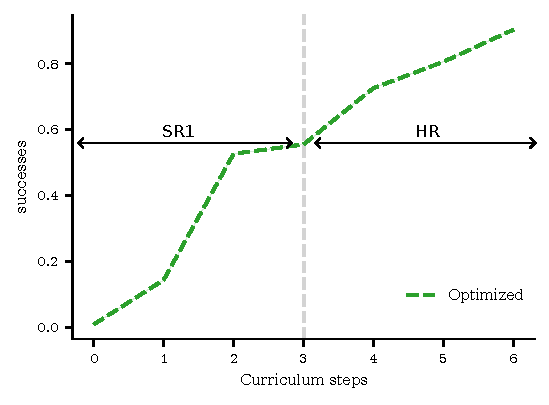
\includegraphics[width=\linewidth]{assets/optimized_switch.pdf}
    \captionof{figure}{The Optimized curriculum policy switching interventions from Soft Reset 1 (SR1 moves the agent one step back) to Hard Reset (HR resets the agent back to the start).}
\end{center}\end{minipage}

\section{Experiments}

\subsection{Curriculum Policies}

\subsubsection{Back}

\begin{itemize}
    \item The Back$_x$ curriculum policy always resets the agent by a constant number of $x$ steps (we tested $x\in[1,9]$)
\end{itemize}

\subsubsection{Incremental}

\begin{itemize}
    \item The Incremental curriculum policy gradually changes from exploration to exploitation
    \item We define Incremental$_x$ to reset the agent by $\lceil \frac{1}{2^x} \cdot n \rceil$ steps during the $n^{\text{th}}$ curriculum step
    \item The parameter $x$ can be adjusted for environments of different size or complexity (we tested $x\in[0,4]$)
\end{itemize}

\subsection{Environments}

\begin{minipage}{\columnwidth}\begin{center}
    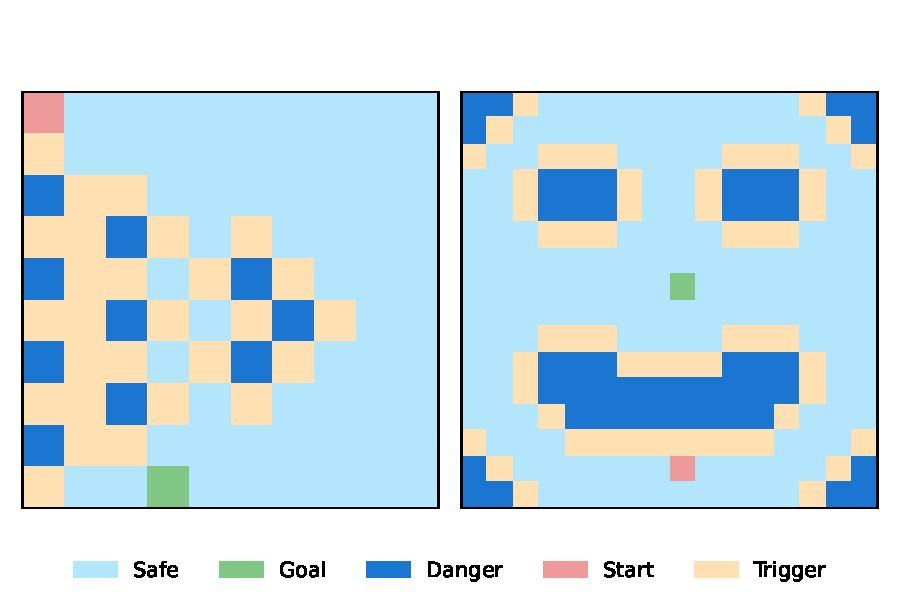
\includegraphics[width=\linewidth]{assets/maps.pdf}
    \captionof{figure}{The Frozen Lake environment used in the paper \cite{Turchetta2020SafeRL} on the left (size 10x10) and our Frozen Smiley environment on the right (size 16x16). Interventions are triggered at distance = 1 from holes.}
\end{center}\end{minipage}
\vspace{1em}

\section{Results}

\begin{itemize}
    \item For all policies with teacher interventions the agent was kept safe during training
    \item Both the Back and the Incremental curriculum policy perform better than the Optimized one
    \item For Back, with increasing environment size and longer paths, it is beneficial to increase reset steps
    \item For Incremental, increasing the reset steps more slowly to allow for longer exploration is advantageous in larger environments
\end{itemize}

\begin{minipage}{\columnwidth}\begin{center}
    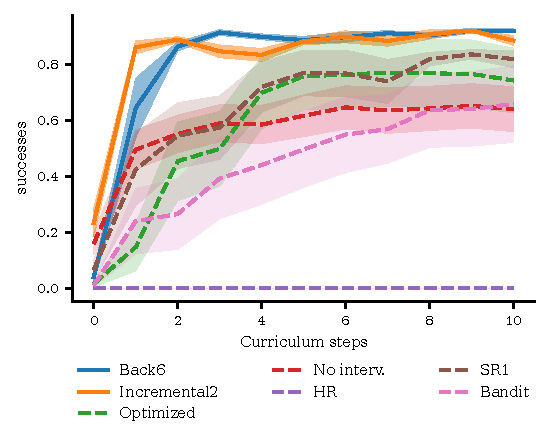
\includegraphics[width=\linewidth]{assets/small_successes.pdf}
    \captionof{figure}{Success rates of different curriculum policies on the Frozen Lake environment. For our policies, the best found parameters $x$ are used.}
\end{center}\end{minipage}
\vspace{1em}

\begin{minipage}{\columnwidth}\begin{center}
    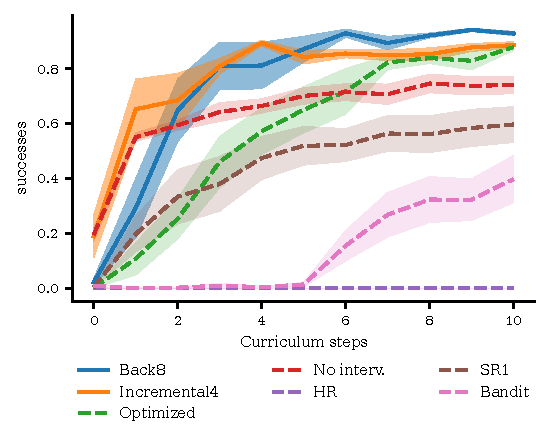
\includegraphics[width=\linewidth]{assets/16x16_successes.pdf}
    \captionof{figure}{Success rates of different curriculum policies on the Frozen Smiley environment. For our policies, the best found parameters $x$ are used.}
\end{center}\end{minipage}
\vspace{1em}

\begin{minipage}{\columnwidth}\begin{center}
    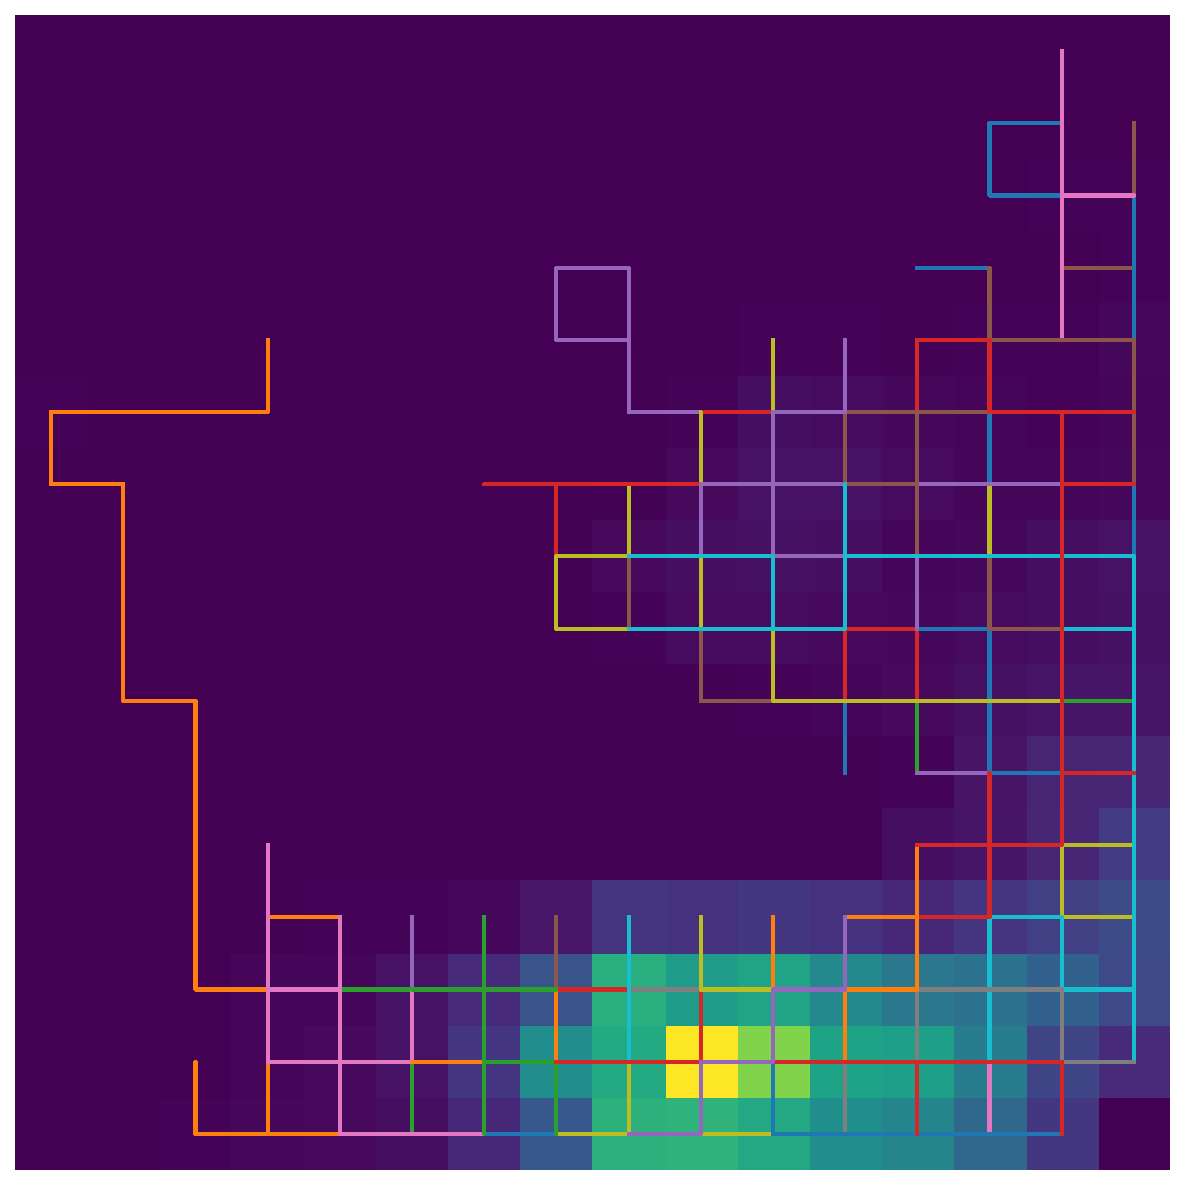
\includegraphics[width=0.48\linewidth]{assets/trajectories0.pdf}
    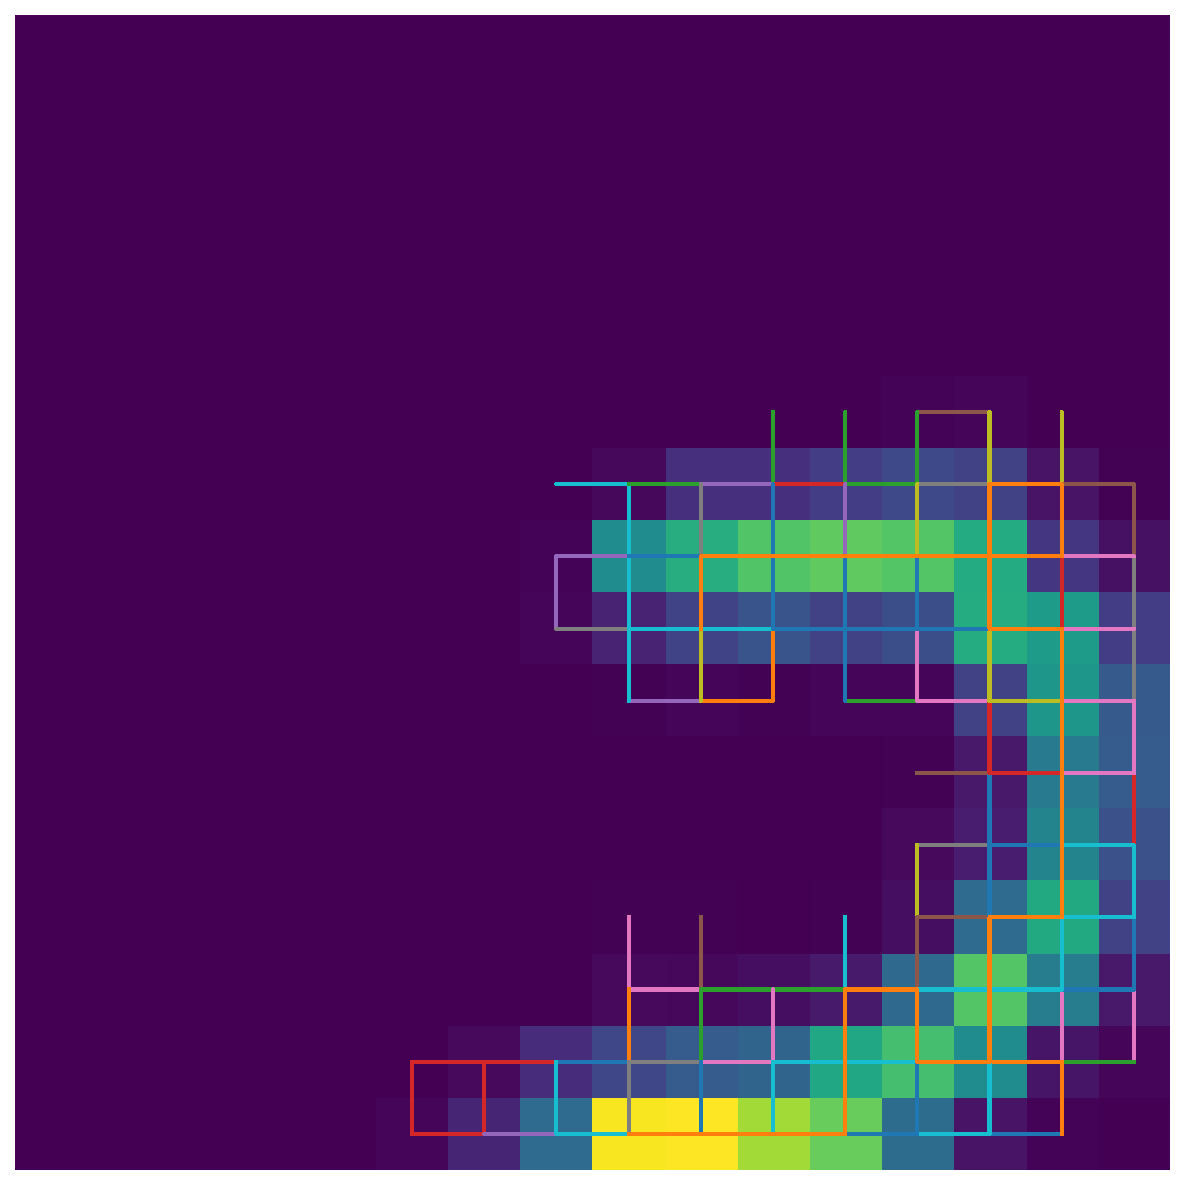
\includegraphics[width=0.48\linewidth]{assets/trajectories6.pdf}
    \captionof{figure}{Exemplary trajectories for the Frozen Smiley environment with the Optimized policy. The lines represent the steps taken, while the background shows a heatmap of the student's positions. The trajectories show a progression from the first curriculum step (left) to a later step (right).}
\end{center}\end{minipage}

%----------------------------------------------------------------------------------------
%	CONCLUSIONS BOX
%----------------------------------------------------------------------------------------

%\section*{} % this dummy section draws a horizontal line above conclusions
\vspace{2cm}
\begin{tcolorbox}[width=0.95\linewidth,colback={conclusion},frame empty,boxsep=1cm]
\section{Conclusions}

\begin{itemize}
    \item For the Frozen environments, our curriculum policies outperform the Optimized one
    \item Larger environments require a longer exploration phase and more reset steps
    \item The original HR, SR and Bandit policies do not generalize well to larger environments
    \item Defining reset transitions which keep the student safe is easier than defining suitable trigger states
    \item This could become a problem when the state space is complex, dynamic or just partly observable
\end{itemize}

\end{tcolorbox}

%----------------------------------------------------------------------------------------
%	OUTLOOK
%----------------------------------------------------------------------------------------

\section{Outlook}

\color{primary}
\begin{itemize}
    \item Apply the method to \mbox{OpenAI's} Safety Gym
    \item Increase the amount of available interventions for the Optimized curriculum policy
    \item Evaluate how well different curriculum policies generalize to dynamic or random environments
\end{itemize}
\color{Black}

%----------------------------------------------------------------------------------------
%	REFERENCES
%----------------------------------------------------------------------------------------
\singlespacing
\small
\nocite{*} % Print all references regardless of whether they were cited in the poster or not
\bibliographystyle{plainurl} % Plain referencing style
\bibliography{literature} % Use the bibliography file literature.bib

%----------------------------------------------------------------------------------------

\end{multicols}
\end{document}